\documentclass[11pt]{article}
% Suppress the output-path-dependent pdfTeX trailer identifier.
% SOURCE_DATE_EPOCH fixes the metadata dates for portable byte reproduction.
\pdftrailerid{}
\usepackage[T1]{fontenc}
\usepackage{lmodern}
\usepackage{amsmath,amssymb,amsthm,mathtools,mathrsfs}
\usepackage[a4paper,margin=27mm]{geometry}
\usepackage{microtype,booktabs,array,graphicx,placeins,flafter}
\usepackage{tikz}
\usetikzlibrary{arrows.meta,calc,positioning}
\usepackage{xr}
\usepackage[colorlinks=true,linkcolor=blue!45!black,citecolor=blue!45!black,urlcolor=blue!45!black]{hyperref}
\urlstyle{same}
\hypersetup{pdftitle={Secondary Saturation and Cusp Geometry at Cancelling Double Grazing},pdfauthor={Haibo Lu}}
\usepackage[nameinlink,noabbrev]{cleveref}
\externaldocument[main-]{main-reference-labels}
\newtheorem{theorem}{Theorem}[section]
\newtheorem{proposition}[theorem]{Proposition}
\newtheorem{lemma}[theorem]{Lemma}
\newtheorem{corollary}[theorem]{Corollary}
\theoremstyle{definition}
\newtheorem{definition}[theorem]{Definition}
\theoremstyle{remark}
\newtheorem{remark}[theorem]{Remark}
\numberwithin{equation}{section}
\newcommand{\R}{\mathbb R}
\newcommand{\sgn}{\operatorname{sgn}}
\newcommand{\id}{\operatorname{id}}
\newcommand{\Fl}{\operatorname{Fl}}
\newcommand{\eps}{\varepsilon}
\newcommand{\bsc}{\widehat{\beta}}
\newcommand{\dsc}{\widehat d}
\newcommand{\smallO}{\mathrm{o}}
\newcommand{\bigO}{\mathrm{O}}
\title{Secondary Saturation and Cusp Geometry\\at Cancelling Double Grazing}
\author{Haibo Lu\\[2pt]
\small Shanghai Institute of Technology, Shanghai 201418, China\\
\small Corresponding author: \href{mailto:luhaibo1985@gmail.com}{luhaibo1985@gmail.com}\\
\small ORCID: \href{https://orcid.org/0009-0000-2717-5968}{0009-0000-2717-5968}}
\date{}
\makeatletter
\renewcommand{\@maketitle}{%
  \begin{center}
    {\Large Secondary Saturation and Cusp Geometry\\
    at Cancelling Double Grazing\par}
    \vspace{5pt}
    {\normalsize Supplement to\\
    \emph{Cyclicity Six and Saturation Geometry at Cancelling Double Grazing}\par}
    \vspace{5pt}
    {\normalsize Haibo Lu\par}
    {\small Shanghai Institute of Technology, Shanghai 201418, China\par}
    {\small Corresponding author:
    \href{mailto:luhaibo1985@gmail.com}{luhaibo1985@gmail.com}\par}
    {\small ORCID: \href{https://orcid.org/0009-0000-2717-5968}{0009-0000-2717-5968}\par}
    \vspace{5pt}
    {\small Mathematical supplement\par}
  \end{center}
  \vspace{6pt}}
\makeatother
\begin{document}
\maketitle
\begin{abstract}
This supplement resolves the corner of the principal-scale saturation
domain where three of the four limiting roots tend to zero. We consider
a semistable limit cycle with two cancelling quadratic grazings whose active
sides agree under transverse transport, with positive first passage strength
$B$ and negative closing curvature.
The strength sum and a secondary scale tend to zero independently.
Necessary bounds hold in every admissible family. In a fixed full-rank
unfolding, the closures of the rescaled six-cycle domains converge in
Hausdorff distance to the coefficient set of cubics with three nonnegative
roots of sum one; every compact subset of its interior is realized
uniformly for all sufficiently small independent scale pairs.
For positive closing offset $a=R(0)$, six-cycle sequences tending to the
reference satisfy the sharp bound $\limsup a/(-b)^3\le4/(27B^2)$, where
$b$ is the multiplier defect. For positive offset we realize six simple
cycles, with one negative and five positive fixed points on the transverse
section. The triple-root endpoint continues to an ordinary cusp.
Near this cusp, the common return interval contains four or six simple cycles
off the fold curves, five distinct cycles on the fold arcs away from the
cusp, one double, and four distinct cycles at the cusp, one triple.
\end{abstract}
\noindent\textbf{Keywords.} Grazing bifurcation; Poincar\'e return maps;
cyclicity; multiple limit cycles; cusp bifurcations.
\par\smallskip
\noindent\textbf{Mathematics Subject Classification.}
Primary 34C23; Secondary 34A36, 34C25, 37G15.
\par\smallskip
\section{Introduction}\label{sup:introduction}

A semistable limit cycle of a continuous piecewise smooth planar system may
have two spatially separated quadratic grazings, with both active sides
agreeing after transport to one transverse section. Each tangency adds a term
of order $q^{3/2}$ to the return map. When the leading coefficients of the two
terms cancel and the closing curvature is nonzero, the displacement has a
double zero at the reference parameter, but nearby return maps can have six
simple fixed points. The companion paper~\cite{main2026} determines the
cyclicity and the saturation domain at the principal scale. Here we study
smaller scales at a boundary of that domain.

The positive cluster at the principal scale is described by a quartic with
four nonnegative roots of sum one. When its quadratic coefficient tends to
zero, three roots approach zero and the fourth approaches one. Their next
coefficient region is cubic. A polynomial rescaling suggests this cubic, but
does not control the return map: the secondary scale can vanish at any rate
relative to the strength sum, and critical points can approach the moving
second threshold. The proof below uses divisions made before either scale
vanishes and slope estimates near that threshold.

We work with positive reference first passage strength $B$ and negative
reference closing curvature $-C$, where $B,C>0$. In terms of the offset
$a=R(0)$, the multiplier defect $b$, the strength sum $m$ and the threshold
separation $\delta$, the secondary weights are
\[
 m=\mu,\qquad b=-\mu^2\sigma,\qquad
 \delta=\mu^3\sigma^2d,\qquad a=\mu^4\sigma^3\alpha.
\]
Both $\mu$ and $\sigma$ are positive and independently small. The limiting
cubic is $z^3-z^2+(3Bd/2)z+\alpha$. Its coefficient region
$\mathcal C_B$ consists of cubics with three nonnegative roots of sum one.
Proposition~\ref{corner:complete-cluster-set} proves that this is exactly
the secondary cluster set and the Hausdorff limit of the six-cycle domains.
Necessity holds in every admissible family; realization uses the standard
unfolding of~\cite{main2026}.

Six-cycle configurations with positive offset occur on a finer offset scale.
With $h=-b$, Proposition~\ref{corner:secondary-bounds} proves the sharp
necessary bound $\limsup a/h^3\leq4/(27B^2)$.
Proposition~\ref{corner:positive-offset-realization} realizes every compact
interior set of the associated parameters by six simple cycles, one with
$q<0$ and five with $q>0$.

At the triple-root endpoint $(\alpha,d)=(-1/27,2/(9B))$,
Theorem~\ref{thm:actual-cusp} constructs an ordinary cusp for every
sufficiently small independent pair $(\mu,\sigma)$.
Lemma~\ref{corner:all-roots} locates every other root in the same interval
$I$. The three simple roots outside the cluster convert the local cubic counts
into the complete four/six-cycle diagram, including its folds and cusp.

The $q^{3/2}$ passage and the composition with regular transitions are
classical~\cite{dibbc2001,nordmark2002}; we use the root-profile form
established in~\cite[Section~2]{main2026}. The Malgrange
preparation theorem~\cite[Chapter~IV, Section~2, Theorem~2.1 and Note~(1), p.~95]{golubitsky1973} is applied after the
multiple root has been located away from both thresholds, where the
displacement is smooth in $q$.

Section~\ref{sup:setting} recalls the setting and the results
of~\cite{main2026} used here. Section~\ref{corner:section} passes from the
quartic corner to the cubic domain through divisions, necessary bounds and
root charts. Section~\ref{sup:positive} treats configurations with positive
offset. Section~\ref{sup:cusp} first locates all roots in $I$ and then unfolds
the secondary triple root.

\section{Setting and results from the companion paper}\label{sup:setting}

We recall the setting of~\cite{main2026} and the estimates used below.

\subsection{Hypotheses and return-map controls}

We use the admissible families
of~\cite[Definition~\ref*{main-def:admissible-family}]{main2026}, with their
two matched quadratic contact boxes, transverse ports and inactive regular
connections; both active sides agree after transport to one transverse section.
The regular transitions are increasing in positive penetration coordinates,
with common positive derivative margins.
On a fixed interval $I=(-q_0,q_0)$ the composition is the first
return map: it makes one turn, with no additional seam crossing or earlier
section hit. Its common open domains include the grazing thresholds and the
closure of a slightly larger interval. The return tube and the transport
through nonidentity connections are given
in~\cite[Lemma~\ref*{main-lem:common-tube} and
Proposition~\ref*{main-prop:field-recognition}]{main2026}.

In the transported transverse coordinate, put
\begin{equation}\label{sup:return}
 Q(q)=\delta+\Gamma_2(\Gamma_1(q)-\delta),\qquad
 P(q)=R(Q(q)),\qquad D(q)=P(q)-q.
\end{equation}
The passages are increasing $C^1$ diffeomorphisms and
\begin{equation}\label{sup:passage}
 \Gamma_\nu(q)=q+A_\nu q_+^{3/2}
       +\tfrac34A_\nu^2q_+^2
       +q_+^{5/2}L_\nu(\sqrt{q_+},\lambda),\qquad q_+=\max(q,0),
\end{equation}
with smooth signed-root profiles. More precisely,
$\Gamma_\nu(r^2)=g_\nu(r)^2$ for $r>0$,
$g_\nu(0)=0$, $g_\nu'(0)=1$ and
$\iota g_\nu\iota=g_\nu^{-1}$, where $\iota(r)=-r$.
Set
\[
 T_\nu(r)=g_\nu(r)/r,\qquad
 \ell_\nu(r)=T_\nu(r)^2+\tfrac r2(T_\nu^2)'(r).
\]
These profiles extend smoothly through zero and
$\Gamma_\nu'(r^2)=\ell_\nu(r)=1+\tfrac32A_\nu r+O(r^2)$.
The return-map controls and the reference signs are
\begin{equation}\label{sup:observations}
 \begin{gathered}
 a=R(0),\qquad b=R'(0)-1,\qquad m=A_1+A_2,\qquad\delta;\\
 a=b=m=\delta=0,\qquad A_1=-A_2=B>0,\qquad
 \tfrac12R''(0)=-C<0.
 \end{gathered}
\end{equation}
We write $p_0$ for the reference value of the remaining parameters.
Here $B,C$ are fixed reference constants, whereas $c(\lambda)=R''_\lambda(0)/2$
and the individual passage strengths retain all parameter dependence.

For necessary estimates, the original parameters are denoted by $p$.
\cite[Lemma~\ref*{main-lem:auxiliary-controls}]{main2026} supplies
independent auxiliary $m,\delta$, with the same closing map, smooth bounded
profiles and the strength identity
$A_1(p,m,\delta)+A_2(p,m,\delta)=m$; restriction gives
the original family. Write $A(p)=A_1(p,0,0)$,
$k(p)=R'_{p,0,0}(0)=1+b>0$ and $c_0(p)=R''_{p,0,0}(0)/2$.
When the controls are independent we write $p=(a,b,\xi)$; the closing
jets $R(0)=a$ and $R'(0)=1+b$ are fixed as $m,\delta$ vary, although
higher closing terms may depend on these controls.

Realization requires the map $\lambda\mapsto(a,b,m,\delta)$ to be a
submersion~\cite[(\ref*{main-eq:rank})]{main2026}. We then use the standard
unfolding $\Lambda(a,b,m,\delta)=\lambda(a,b,m,\delta;\xi_0)$
of~\cite{main2026}, defined on a neighbourhood $\mathcal V\subset\R^4$ of
zero, and the same interval $I$. Write
$N_\lambda(I)=\#\{q\in I:D_\lambda(q)=0\}$. Families with this property are
constructed in~\cite[Proposition~\ref*{main-prop:specified-rank} and
Theorem~\ref*{main-thm:harvesting-realization}]{main2026}. We follow the
conventions of~\cite[Section~2]{main2026}: state
derivatives are taken at fixed parameters, and all profile bounds hold on
common compact reductions.

\subsection{Divisions, curvature and saturation}

We record the results of~\cite{main2026} used below. The closing expansion
is
\begin{equation}\label{sup:closing}
 R(y)=a+(1+b)y+c(\lambda)y^2+y^3S(y,\lambda).
\end{equation}
After one common reduction, choose $r_0>0$ and $v_0=1/4$.
For $0<r\le r_0$, $|v|\le v_0$ and $(m,p)$ in the common small
neighbourhood, put $q=r^2$ and $\delta=r^2v$. Both passages are active,
and \cite[Lemma~\ref*{main-lem:exact-value-division}]{main2026} gives
profiles smooth in signed $(r,m,v,p)$ with
\begin{equation}\label{sup:root-division}
 Q-q=mr^3+\tfrac34m^2r^4+r^5L_0+\delta rH(r,m,v,p),
 \qquad H(0,0,0,p)=\tfrac32A(p).
\end{equation}
For either sign of $q$ and $\delta$, including the thresholds, the same lemma
gives
\begin{equation}\label{sup:global}
 |Q-q-mq_+^{3/2}|\leq K\{m^2q_+^2+q_+^{5/2}
       +|\delta|\sqrt{q_++|\delta|}+|\delta|q_+^{3/2}\}.
\end{equation}
By~\cite[Lemma~\ref*{main-lem:curvature-profile} and
Proposition~\ref*{main-prop:one-fold-graph}]{main2026}, the zeros of $P''$ in
the outer region lie on the separation graph \eqref{corner:curvature-division}.
Its derivative is
$\Delta_r=r\mathcal W$, with $\mathcal W_r$ having a uniform nonzero
margin of sign $c_0/A$;
thus it has at most one positive critical point, which is nondegenerate.
At fixed parameters the curvature factorization is
\[
 P''(r^2)=r^{-3}\mathcal U(r,m,\delta/r^2,p)
                  [\delta-\Delta(r,m,p)],\qquad \sgn\mathcal U=-\sgn A.
\]
For $A>0,c_0<0,m>0$, the critical point satisfies
$r_{\rm c}=-km/(4c_0)+O(m^2)$.
\cite[Lemma~\ref*{main-lem:event-layer}]{main2026} covers the threshold
layer, uniformly up to the thresholds. For positive separation the thresholds
are $0$ and $a_\delta=\Gamma_1^{-1}(\delta)$; in the threshold layer the signs
of $P''$ where no passage, only the first passage, and both passages are
active are $-,+,-$. For any fixed $L\geq2$, these signs hold for
$q\leq L\delta$ away from the thresholds. In the active regions,
$|Q''|\geq\kappa_L\delta^{-1/2}$, uniformly in the one-sided approach to
each threshold. Together with the
graph, they give the bound of six fixed points on
$I$~\cite[Proposition~\ref*{main-prop:common-count}]{main2026}.

If the bound is attained, \cite[Lemma~\ref*{main-sat:saturation}]{main2026}
gives $m,\delta,h=-b>0$, two simple zeros $\zeta_1<\zeta_2$ of $P''$ in the
outer region, and the slopes recorded in \eqref{corner:saturation-slopes}.
The five curvature blocks have signs $-,+,-,+,-$ and each contains one
zero $t_j$ of $D_q$, with successive extremal values of signs
$+,-,+,-,+$. Every fixed point is simple as a $C^1$ zero.
Finally \cite[Proposition~\ref*{main-sat:weighted-confinement}]{main2026}
gives the weighted confinement
\begin{equation}\label{sup:confinement}
 0<h\leq Km^2,\qquad 0<\delta\leq Km^3,\qquad
 |a|\leq Km^4,\qquad \max_{D(q)=0}|q|\leq Km^2.
\end{equation}
The next section refines this confinement by evaluating the slope on the
separation graph.

\section{The two-scale secondary saturation domain}\label{corner:section}

We determine the coefficient region reached when three roots of the
principal quartic collapse to zero. A division of the slope gives the finer
necessary scales; the joint return quotient and root charts then identify
the region and realize its interior.
Throughout this section we use the setting and conventions of
Section~\ref{sup:setting}.

\subsection{The quartic corner and its cubic limit}

The principal-scale coordinates
of~\cite[Section~\ref*{main-subsec:four-root-limit}]{main2026} are
\[
 A_4=\frac{C^3a}{m^4},\qquad S_4=\frac{Ch}{m^2},\qquad
 T_4=\frac{3BC^2\delta}{2m^3},\qquad x=\frac{C\sqrt q}{m},
 \qquad h=-b.
\]
Write $e_j$ for the elementary symmetric polynomial of degree $j$, and set
\[
 \Phi_{A,S,T}(x)=A-Sx^2+x^3-x^4+Tx,\qquad
 \mathcal K_4=\{(-e_4,e_2,e_3):r_i\geq0,\ \textstyle\sum_{i=1}^4r_i=1\}.
\]
Thus $\Phi_{A_4,S_4,T_4}=-\prod_{i=1}^4(x-r_i)$ for a point in
$\mathcal K_4$. We abbreviate this polynomial by $\Phi$.
The corner $S_4\to0$ of $\mathcal K_4$ explains the next scale.
Order the four roots and write $u=r_1+r_2+r_3$, $v=r_1r_2+r_1r_3+r_2r_3$,
$w=r_1r_2r_3$. Since $r_4=1-u$,
\[
 S_4=(1-u)u+v,\qquad T_4=(1-u)v+w,\qquad -A_4=(1-u)w.
\]
Along any sequence with $S_4\to0^+$, the largest root tends to one and
$u/S_4\to1$. After passing to a subsequence, $r_i/S_4\to z_i\ge0$ for
$i=1,2,3$, with $\sum_{i=1}^3z_i=1$. Along this subsequence,
$(A_4/S_4^3,T_4/S_4^2)\to(-e_3(z),e_2(z))$.
Conversely, taking small roots $t z_i$ with $\sum z_i=1$
and large root $1-t$ realizes every such limit; here
$S_4=t-t^2(1-e_2(z))\sim t$.

Set $\sigma_4=S_4$ and write $A_4=\sigma_4^3\alpha$,
$T_4=\sigma_4^2T_3$, and $x=\sigma_4z$. Then
\[
 \Phi(\sigma_4z)/\sigma_4^3
 =\alpha-z^2+z^3+T_3 z-\sigma_4z^4.
\]
The polynomial identity identifies a candidate cubic. Transferring it to
the return map when $h=-b=o(m^2)$ requires a division before either scale
vanishes: an additive error $o(m^2)$ in the slope would not control $h$.
The necessary estimates use sequences whose original parameters, including
all remaining parameters, tend to the reference of Section~\ref{sup:setting}.

\subsection{Slope division and necessary bounds}

The finer scales are forced by the slope at the first zero of $P''$ in the
outer region and by the extrema of the displacement. We begin with a division
of the slope on the separation graph.

For a return with six fixed points, let $a_\delta=\Gamma_1^{-1}(\delta)$ be the
second threshold. By~\cite[Lemma~\ref*{main-sat:saturation}]{main2026} each
open curvature block contains one zero $t_j$ of $D_q$, with extremal signs
$+,-,+,-,+$, and
\begin{equation}\label{corner:saturation-slopes}
 D_q(0)<0,\quad D_q(a_\delta)>0,\quad D_q(\zeta_1)<0,\quad D_q(\zeta_2)>0.
\end{equation}
Here \(\zeta_1<\zeta_2\) are the two zeros of \(P''\) in the outer region; in
particular
\(m,\delta,h=-b\) are positive.

The separation graph of~\cite[Section~3]{main2026} is
\begin{equation}\label{corner:curvature-division}
 \begin{aligned}
 \delta=\Delta(r,m,p)&=r^2\{mH_\Delta(r,m,p)+rB_\Delta(r,p)\},\\
 H_\Delta(0,0,p)&=\frac2{A(p)},\qquad
 B_\Delta(0,p)=\frac{16c_0(p)}{3k(p)A(p)}.
 \end{aligned}
\end{equation}
Here $B_\Delta,H_\Delta$ are smooth profiles.

\begin{lemma}[Slope on the separation graph]
\label{corner:graph-slope}
After a common reduction there are jointly smooth profiles $H_D,B_D$
such that
\begin{equation}\label{corner:exact-graph-slope}
 \left.D_q(r^2,p,m,\delta)\right|_{\delta=\Delta(r,m,p)}
 =b+r\{mH_D(r,m,p)+rB_D(r,p)\},
\end{equation}
with
\begin{equation}\label{corner:graph-slope-coefficients}
 H_D(0,0,p)=3k(p),\qquad B_D(0,p)=6c_0(p).
\end{equation}
\end{lemma}

\begin{proof}
Use the signed-root profiles
of~\cite[Section~3]{main2026}.
With $\delta=r^2v$, the expression
\[
 D_q(r^2)=R'(Q)\ell_2(r\sqrt{T_1(r)^2-v})\ell_1(r)-1
\]
extends smoothly in $(r,m,v,p)$ on a common box.  At $r=0$ it equals
$b$ for all small $m,v$.  Hadamard division in $r$ therefore gives a
smooth function $\mathcal T$ such that $D_q-b=r\mathcal T$.
The first passage derivatives give
\[
 \ell_\nu(u)=1+\tfrac32 A_\nu u+O(u^2).
\]
Consequently, at the root boundary,
\[
 \mathcal T(0,m,v,p)
 =\tfrac32 k(p)
   \{A_1(p,m,0)+A_2(p,m,0)\sqrt{1-v}\}.
\]
The aligned strength identity yields the linear terms
$\tfrac32km+\tfrac34kAv$.  On $m=v=0$, finite cancellation gives
$D_q-b=2c_0r^2+O(r^3)$.  Joint Taylor division thus gives
\begin{equation}\label{corner:fixed-control-slope-expansion}
 \mathcal T
 =2c_0r+\tfrac32km+\tfrac34kAv
       +O\bigl((|r|+|m|+|v|)^2\bigr),
\end{equation}
with a uniform smooth remainder.

Now substitute the graph
$v=V(r,m,p)=mH_\Delta+rB_\Delta$ in $\mathcal T$, and call the resulting
smooth function $\mathcal T_\Delta(r,m,p)$. Formula
\eqref{corner:fixed-control-slope-expansion} gives
\[
 \mathcal T_\Delta(0,0,p)=0,\qquad
 \partial_m\mathcal T_\Delta(0,0,p)=3k,\qquad
 \partial_r\mathcal T_\Delta(0,0,p)=6c_0.
\]
Define $B_D(r,p)=\mathcal T_\Delta(r,0,p)/r$ by smooth division and
\[
 H_D(r,m,p)=\int_0^1\partial_m\mathcal T_\Delta(r,sm,p)\,ds.
\]
Thus $\mathcal T_\Delta=rB_D+mH_D$, proving
\eqref{corner:exact-graph-slope}--\eqref{corner:graph-slope-coefficients}.
\end{proof}

For $\delta>0$, $q\geq0$, the global passage estimate
\eqref{sup:global} gives
\begin{align}
 |D(q)-a|\leq K\{&
 hq+q^2+mq^{3/2}+m^2q^2+q^{5/2}\notag\\
 &+\delta\sqrt{q+\delta}+\delta q^{3/2}\},
 \qquad h=-b>0.                         \label{corner:global-comparison}
\end{align}
Indeed $0\leq Q(q)\leq Kq$ uniformly.  Below $a_\delta$ this follows from
$Q=\Gamma_1(q)$; above $a_\delta$, positivity and a common bound
$\Gamma_2(y)\leq Ky$, with $K\geq1$, give
$\delta+\Gamma_2(\Gamma_1(q)-\delta)\leq K\Gamma_1(q)$.
Insert this bound in the closing expansion
\eqref{sup:closing} and apply
\eqref{sup:global}.

\begin{proposition}[Secondary necessary bounds]
\label{corner:secondary-bounds}
\label{corner:sharp-positive-offset}
\label{corner:positive-offset-bound}
There is a constant $K$ such that, for parameters sufficiently close to the
reference in this sign case, every return with six fixed points satisfies,
with $h=-b$,
\begin{equation}\label{corner:strong-bounds}
 0<h\leq Km^2,\qquad
 0<\delta\leq K\frac{h^2}{m},\qquad
 -K\frac{h^3}{m^2}\leq a\leq Kh^3.
\end{equation}
More precisely, with $k=1-h$ and the current first passage strength
$A_1(\lambda)$,
\begin{equation}\label{corner:finite-positive-offset-bound}
 a<\frac{4h^3}{27k^2A_1(\lambda)^2}+Kh^4.
\end{equation}
Along every six-fixed-point sequence tending to the reference, this gives
\begin{equation}\label{corner:sharp-positive-offset-limsup}
 \limsup\frac{a}{h^3}\leq\frac{4}{27B^2}.
\end{equation}
\end{proposition}

The leading term in~\eqref{corner:finite-positive-offset-bound} agrees with
Simpson and Meiss's fold value $4(1-\Xi)^3/(27\gamma^2)$ for the truncated
return~\cite[arXiv version, Eq.~(72)]{simpsonmeiss2008}, with $h=1-\Xi$ and
$\gamma=kA_1(\lambda)$. Here the bound retains $Kh^4$ and is necessary for
arbitrary six-cycle configurations; Proposition~\ref{corner:positive-offset-realization}
proves sharpness by sequences approaching the endpoint.

\begin{proof}
\cite[Proposition~\ref*{main-sat:weighted-confinement}]{main2026} gives
\(h\le Km^2\).
Put \(\rho_i=\sqrt{\zeta_i}\).

The root coordinate $\rho_1$ of the first curvature zero lies below the
graph's unique positive critical point, whose expansion is
\[
 \rho_1<r_{\rm c}
 =-\frac{k(p)m}{4c_0(p)}+O(m^2).
\]
Uniformly for $0<r\leq r_{\rm c}$, the slope profiles satisfy
\[
 mH_D+rB_D\geq c_*m,\qquad c_*>0.
\]
To check the margin, divide by $m$ and use
\eqref{corner:graph-slope-coefficients}: the limiting minimum on this
interval is
$3k+6c_0[-k/(4c_0)]=3k/2>0$.
The negative slope at $\zeta_1$ therefore yields
\[
 \rho_1\leq K\frac hm,\qquad
 \zeta_1\leq K\frac{h^2}{m^2}.
\]
Using \eqref{corner:curvature-division} at $\rho_1$, where
$mH_\Delta+\rho_1B_\Delta=O(m)$, proves
$\delta\leq Kh^2/m$.

For the upper offset bound, the negative minimum $t_2=r_2^2$ lies
where only the first passage is active, so that $Q=\Gamma_1(q)$. Uniform
passage and closing expansions at fixed parameters give
\[
 D(r^2)=a-hr^2+(1-h)A_1r^3+O(r^4),\qquad
 D_q(r^2)=-h+\tfrac32(1-h)A_1r+O(r^2).
\]
The coefficient $\tfrac32(1-h)A_1$ has a uniform positive lower bound.
After reducing the state interval, the $O(r_2^2)$ term is absorbed in
that linear term. Thus $D_q(t_2)=0$ first gives $r_2=O(h)$ and then
\[
 r_2=\frac{2h}{3kA_1(\lambda)}+O(h^2).
\]
The value expansion therefore yields
\begin{equation}\label{corner:first-minimum-sharp}
 D(t_2)=a-\frac{4h^3}{27k^2A_1(\lambda)^2}+O(h^4).
\end{equation}
Its strict negativity proves \eqref{corner:finite-positive-offset-bound}
and the coarse upper bound in \eqref{corner:strong-bounds}.
Since $k\to1$ and $A_1(\lambda)\to B$ along a converging sequence,
it also proves \eqref{corner:sharp-positive-offset-limsup}.
Thus $a\leq4h^3/(27B^2)+o(h^3)$.

For the lower bound use the third extremum $t_3\in(a_\delta,\zeta_1)$.
It has $D(t_3)>0$ and $t_3\leq Kh^2/m^2$.  Substitute this and
$\delta\leq Kh^2/m$ in \eqref{corner:global-comparison}.
The terms $ht_3$ and $mt_3^{3/2}$ are $O(h^3/m^2)$.
The term $t_3^2$ is bounded by that size times $h/m^2$, which is
bounded by the first estimate.  The higher aligned terms are smaller.
Finally,
\[
 \delta\sqrt{t_3+\delta}
 \leq K\left(\frac{h^3}{m^2}+\frac{h^3}{m^{3/2}}\right).
\]
The remaining separation term is smaller as well. Thus
$|D(t_3)-a|\leq Kh^3/m^2$, proving the lower offset bound.

\end{proof}


\subsection{The joint secondary quotient}

In the standard unfolding introduce
\begin{equation}\label{corner:weights}
 m=\mu,\qquad b=-\mu^2\sigma,\qquad
 \delta=\mu^3\sigma^2d,\qquad a=\mu^4\sigma^3\alpha,
 \qquad \mu,\sigma>0.
\end{equation}
These weights give $\sigma_4=S_4=C\sigma$ and $T_3=3Bd/2$.
The weight map has determinant $-\mu^9\sigma^5$ with rows
$(m,b,a,\delta)$ and columns $(\mu,\sigma,\alpha,d)$.
Here $h=\mu^2\sigma$ and the secondary positive state coordinate is
\[
 q=\mu^2\sigma^2z^2.
\]
The threshold layer has relative size $\delta/q=\mu d/z^2$, so on fixed
positive $z$-intervals both passages are active for small $\mu$, even when
$\sigma$ tends to zero independently.

\begin{definition}[Secondary saturation domain]
\label{def:actual-secondary-domain}
Use the neighbourhood $\mathcal V$, the standard unfolding $\Lambda$ and the
count $N_\lambda(I)$ of Section~\ref{sup:setting}.
Let $w_{\mu,\sigma}(\alpha,d)=(a,b,m,\delta)$ be given by
\eqref{corner:weights}. The secondary saturation domain is
\[
 \mathscr S_{\mu,\sigma}
 =\{(\alpha,d)\in\R^2:w_{\mu,\sigma}(\alpha,d)\in\mathcal V,
       N_{\Lambda(w_{\mu,\sigma}(\alpha,d))}(I)=6\}.
\]
\end{definition}

Define the compact set
\begin{equation}\label{corner:CB}
 \mathcal C_B=
 \left\{\left(-r_1r_2r_3,\,
       \frac{2(r_1r_2+r_1r_3+r_2r_3)}{3B}\right):
       r_i\geq0,\quad r_1+r_2+r_3=1\right\}.
\end{equation}

We use Euclidean distance for the Hausdorff distance $d_H$ between compact
coefficient sets. The quotient below connects the cubic region to the return
map, with no relation between $\mu$ and $\sigma$. Further charts and
estimates of critical points then account for the remaining roots and the
boundary.

\begin{lemma}[Joint secondary quotient]
\label{corner:joint-quotient}
On every compact positive $z$-interval and bounded set of rescaled
parameters, the function
\[
 \mathcal F_{\mu,\sigma}(z;\alpha,d)
 =\frac{D(\mu^2\sigma^2z^2)}{\mu^4\sigma^3}
\]
extends jointly smoothly to signed $(\mu,\sigma)$ near $(0,0)$. There is a
jointly smooth profile $E$ such that
\begin{equation}\label{corner:joint-limit}
 \mathcal F_{\mu,\sigma}
 =\alpha-z^2+z^3+\tfrac32 Bdz-C\sigma z^4
       +\mu E(\mu,\sigma,z,\alpha,d).
\end{equation}
Every prescribed finite collection of mixed derivatives is bounded on
closed reductions. The extension equals the rescaled displacement for
$\mu,\sigma>0$.
\end{lemma}

\begin{proof}
The root-profile division
\eqref{sup:root-division}, before any weights are imposed, gives
\begin{equation}\label{corner:exact-Q-division}
 Q-q=mr^3+\tfrac34m^2r^4+r^5L_0+\delta rH(r,m,v,p),
 \qquad v=\delta/r^2,\qquad H(0,0,0,p_0)=\tfrac32B.
\end{equation}
Set $r=\mu\sigma z$ and $v=\mu d/z^2$.  Define
\begin{align}
 V&=z^3+dzH+\mu\sigma^2z^5L_0
                    +\tfrac34\mu^2\sigma z^4,\notag\\
 Y&=z^2+\mu^2\sigma V.                  \label{corner:VY}
\end{align}
These are jointly smooth for positive $z$ in a compact interval,
including signed auxiliary $\mu,\sigma$, and satisfy
$Q-q=\mu^4\sigma^3V$, $Q=\mu^2\sigma^2Y$ for positive scales.
The closing expansion gives
\begin{equation}\label{corner:exact-residual}
 \mathcal F_{\mu,\sigma}
 =\alpha+V-Y+c(\lambda)\sigma Y^2
       +\mu^2\sigma^3Y^3S(\mu^2\sigma^2Y,\lambda).
\end{equation}
At $\mu=0$, all four controls in
\eqref{corner:weights} vanish, for every small $\sigma$.
Because $\xi$ is fixed, $c=-C$ and $H=3B/2$ there.  The restriction of
\eqref{corner:exact-residual} to $\mu=0$ is therefore exactly
$\alpha-z^2+z^3+(3B/2)dz-C\sigma z^4$.
Taylor integral division in $\mu$ proves \eqref{corner:joint-limit}
and the mixed bounds.
\end{proof}

For a dependent family whose original parameters tend to the reference,
if $\mu_n,\sigma_n\to0^+$ and $(\alpha_n,d_n)$ stay bounded, the same
identity gives, on every compact positive $z$ interval,
\begin{equation}\label{corner:sequence-limit}
 \frac{D_n(\mu_n^2\sigma_n^2z^2)}
           {\mu_n^4\sigma_n^3}
 -\{\alpha_n-z^2+z^3+\tfrac32Bd_nz\}\longrightarrow0
\end{equation}
in every prescribed finite state derivative.  Indeed
\eqref{corner:exact-Q-division} and \eqref{corner:exact-residual} still
hold along the sequence, with its original remaining parameters retained.
Their profiles converge to their reference values, and all their
$z$ derivatives are controlled by the same smooth root expressions.

\subsection{Charts for the remaining roots}

The following charts supply the remaining roots both in the secondary
interior and in the positive-offset configurations of
Section~\ref{sup:positive}.

\begin{lemma}[Charts for the remaining roots]
\label{corner:realization-charts}
In the standard unfolding, for bounded $\alpha,d$ with $d>0$, the following
limits hold in $C^1$ on the indicated compact
state intervals as $\mu,\sigma\to0^+$ independently:
\begin{align}
 \frac{D(\mu^2\sigma^2x)}{\mu^4\sigma^3}
     &\longrightarrow\alpha-x,
       &&x\Subset(-\infty,0),                         \label{corner:negative-small-chart}\\
 \frac{D(-hX/C)}{h^2/C}
     &\longrightarrow X-X^2,
       &&X\Subset(0,\infty),                          \label{corner:negative-large-chart}\\
 \frac{D(\mu^2X)}{\mu^4}
     &\longrightarrow X^{3/2}-CX^2,
       &&X\Subset(0,\infty).                          \label{corner:positive-large-chart}
\end{align}
Convergence is uniform when the rescaled parameters range over a compact
set.
\end{lemma}

\begin{proof}
For $q<0$ both passages are exactly inactive because $\delta>0$.
Thus \eqref{sup:closing} gives
$D(q)=a+bq+c(\lambda)q^2+q^3S(q,\lambda)$.
Substituting $q=\mu^2\sigma^2x$ and $q=-hX/C$, using
\eqref{corner:weights}, $h=\mu^2\sigma$ and $c(\lambda)\to-C$,
proves \eqref{corner:negative-small-chart} and
\eqref{corner:negative-large-chart}.

For the positive outer chart set $r=\mu\sqrt X$ and
$v=\mu\sigma^2d/X$ in the root division
\eqref{corner:exact-Q-division}. Here $v\to0$ uniformly on the prescribed
positive compact intervals, so both passages are active in this chart. The division gives
$(Q-q)/\mu^4\to X^{3/2}$ and $Q/\mu^2\to X$ in $C^1$.
In \eqref{sup:closing}, $a/\mu^4=\sigma^3\alpha$,
$b/\mu^2=-\sigma$, $c(\lambda)\to-C$, and the cubic closing remainder
divided by $\mu^4$ tends to zero. This proves
\eqref{corner:positive-large-chart}. Smooth profiles give the stated
$C^1$ uniformity on compact sets of states and rescaled parameters as
$\mu,\sigma\to0^+$ independently.
\end{proof}

\subsection{Critical points and the limiting cubic}

For the necessary limits we again allow dependent controls.
For $d\ge0$, write $T_3=3Bd/2$ and
\[ F_{\alpha,d}(z)=z^3-z^2+T_3 z+\alpha. \]

Necessity requires control at the left endpoint of the positive root
chart. We first place the third and fourth extrema on the secondary
scale. For a positive limit of $d$, separated passage slopes exclude
the threshold layer; when $d\to0$, the third maximum supplies the missing
value estimate.

\begin{lemma}[Limiting critical points]
\label{corner:limiting-critical-states}
Let a sequence in an admissible family tend to its reference,
with six distinct fixed points, $\mu=m\to0^+$ and
$\sigma=-b/m^2\to0^+$. Pass to a subsequence on which the bounded
normalized parameters satisfy $(\alpha,d)\to(\alpha_0,d_0)$.
If $d_0>0$, the third and fourth displacement extrema satisfy
\[
 \frac{\sqrt{t_3}}{\mu\sigma}\longrightarrow
 z_-=\frac{1-\sqrt{1-3T_{3,0}}}3,\qquad
 \frac{\sqrt{t_4}}{\mu\sigma}\longrightarrow
 z_+=\frac{1+\sqrt{1-3T_{3,0}}}3,
 \qquad T_{3,0}=\tfrac32Bd_0,
\]
where $0<T_{3,0}\leq1/3$.  Moreover,
\begin{equation}\label{corner:critical-value-inequalities}
 F_{\alpha_0,d_0}(z_-)\geq0,\qquad
 F_{\alpha_0,d_0}(z_+)\leq0,\qquad \alpha_0\leq0.
\end{equation}
If $d_0=0$, then $\alpha_0=0$.
\end{lemma}

\begin{proof}
Proposition~\ref{corner:secondary-bounds} gives
\[
 -K\leq\alpha\leq K\mu^2,\qquad 0<d\leq K.
\]
Write $\rho_1=\mu\sigma z_c$.  The same bounds control $z_c$.
The graph and slope identities yield
\begin{equation}\label{corner:normalized-curvature}
 d=z_c^2\{H_\Delta+\sigma z_cB_\Delta\}
       =\frac2Bz_c^2+o(1),\qquad
 \frac{D_q(\zeta_1)}h=-1+z_cH_D+\sigma z_c^2B_D
       =-1+3z_c+o(1).
\end{equation}
The strict negative slope gives $\limsup z_c\leq1/3$ and therefore
$d_0\leq2/(9B)$.

We already have $0<t_3<\zeta_1=O(\mu^2\sigma^2)$.
To obtain the same bound for $t_4$, first note that
\begin{equation}\label{corner:larger-curvature-radius}
 \rho_2/\mu\longrightarrow\frac3{8C}.
\end{equation}
In fact $\rho_2=O(\mu)$ by the curvature graph, it is beyond the
positive critical point $r_{\rm c}/\mu\to1/(4C)$ of the graph, and
$\delta/\mu^3=\sigma^2d\to0$.  Dividing
\eqref{corner:curvature-division} by $\mu^3$ shows that every limit
$w$ of $\rho_2/\mu$ satisfies
\[
 0=w^2\left(\frac2B-\frac{16C}{3B}w\right).
\]
The lower bound supplied by this critical point selects $w=3/(8C)$.
Choose a fixed $Z$ larger than the bound for $z_c$ and large enough
that $-1+3Z/2>0$.  By \eqref{corner:sequence-limit} and the chain rule in the state,
\[
 \frac{D_q(\mu^2\sigma^2Z^2)}h
 =-1+\tfrac32Z+\frac{3Bd}{4Z}+o(1)>0.
\]
For small scales this state lies in $(\zeta_1,\zeta_2)$, by
\eqref{corner:larger-curvature-radius}.  The derivative is strictly
increasing on that interval, so its unique zero $t_4$ lies before
the test state.  Thus both normalized critical states are bounded.

Suppose now that $d_0>0$. We exclude a zero of $D_q$ at
$q=\mu^2\sigma^2z^2$ with $z\to0$ where both passages are active.
Put $y=\Gamma_1(q)-\delta\geq0$. Along this sequence the parameters
and state lie in the common small domain, $A_1\ge B/2$, and $m,\delta>0$.
Since
\[
 \frac{q^{3/2}}{\delta}=\frac{\sigma z^3}{d}\longrightarrow0,
\]
the estimate of~\cite[(\ref*{main-sat:threshold-slope-exclusion})]{main2026} applies and gives
$D_q(q)\geq\kappa\delta/\sqrt q-K(h+q)$.
With the exact substitutions
\[
 \frac{\delta}{\sqrt q\,h}=\frac dz,\qquad
 \frac qh=\sigma z^2,
\]
we obtain, for a constant $c_*>0$,
\begin{equation}\label{corner:event-layer-slope-exclusion}
 \frac{D_q(q)}h\geq-K+c_*\frac dz-K\sigma z^2.
\end{equation}
The right side tends to $+\infty$, which contradicts a zero of $D_q$. The
estimate also holds as $y\to0$, at the second threshold.

The two normalized critical points now remain in a compact subset of
$(0,\infty)$.  Their limits are zeros of
$F'_{\alpha_0,d_0}=3z^2-2z+T_{3,0}$, by
\eqref{corner:sequence-limit}.  Their order on either side of $z_c$,
whose limit is $\sqrt{Bd_0/2}=\sqrt{T_{3,0}/3}$,
selects $z_-,z_+$, respectively; at $T_{3,0}=1/3$ the two
limits agree.  The signs $D(t_3)>0$, $D(t_4)<0$ give
\eqref{corner:critical-value-inequalities}.  The upper offset bound
already gives $\alpha_0\leq0$.

If $d_0=0$, \eqref{corner:normalized-curvature} instead gives
$z_c\to0$, so $z_M=\sqrt{t_3}/(\mu\sigma)\leq z_c\to0$.
At this state \eqref{corner:global-comparison}, divided by
$\mu^4\sigma^3$, gives the explicit bound
\begin{align*}
 \frac{|D(t_3)-a|}{\mu^4\sigma^3}\leq K\{&
 z_M^2+z_M^3+\sigma z_M^4+\mu^2\sigma z_M^4
       +\mu\sigma^2z_M^5\\
 &+dz_M+\sqrt\mu\,d^{3/2}
       +\mu^2\sigma^2d z_M^3\}.
\end{align*}
Every term tends to zero.  Positivity of $D(t_3)$ implies
$\alpha_0\geq0$, and $\alpha\leq K\mu^2$ implies
$\alpha_0\leq0$.  Therefore $\alpha_0=0$.
\end{proof}

\subsection{The complete corner domain}

The limits of the critical points give necessity, while the joint quotient
and the charts of Lemma~\ref{corner:realization-charts} give interior
realization.
The interior of $\mathcal C_B$ consists precisely of parameters for which
$F_{\alpha,d}$ has three distinct positive roots.  Equivalently,
\begin{equation}\label{corner:discriminant}
 \mathcal C_B=
 \left\{(\alpha,d):
 \begin{array}{l}
 \alpha\leq0,\quad d\geq0,\\
 T_3^2-4T_3^3+4\alpha-18T_3\alpha-27\alpha^2\geq0
 \end{array}\right\}.
\end{equation}

\begin{proposition}[Secondary corner domain]
\label{corner:complete-cluster-set}
\label{thm:saturation-geometry}
\label{cor:saturation-domain-limit}
In the fixed sign sector the following statements hold.
\begin{enumerate}
\item
Let parameters in an admissible family tend to the reference.  Suppose each return has six distinct fixed points and
\[
 m\longrightarrow0^+,\qquad
 \sigma=\frac{-b}{m^2}\longrightarrow0^+.
\]
Then the normalized parameters
\begin{equation}\label{corner:normalized-observations}
 \alpha=\frac{a}{m^4\sigma^3}
        =\frac{am^2}{h^3},
 \qquad
 d=\frac{\delta}{m^3\sigma^2}
   =\frac{m\delta}{h^2},\qquad h=-b,
\end{equation}
are bounded, and every cluster point belongs to $\mathcal C_B$.
In particular
\begin{equation}\label{corner:sharp-cluster-bounds}
 \liminf\alpha\geq-\frac1{27},\qquad
 \limsup\alpha\leq0,\qquad
 0\leq\liminf d\leq\limsup d\leq\frac2{9B}.
\end{equation}
If $a\geq0$ eventually, the last upper bound improves to
\begin{equation}\label{corner:nonnegative-offset-bound}
 \limsup d\leq\frac1{6B}.
\end{equation}

\item
Assume~\cite[(\ref*{main-eq:rank})]{main2026} and use the standard
unfolding. For every compact
$\mathcal K\Subset\operatorname{int}\mathcal C_B$, there exist
$\mu_0,\sigma_0>0$ such that, for every
\[
 0<\mu<\mu_0,\qquad 0<\sigma<\sigma_0,\qquad
 (\alpha,d)\in\mathcal K,
\]
the parameters \eqref{corner:weights} give exactly six simple fixed points
in $I$.  If $r_1<r_2<r_3$ are the positive roots of
$F_{\alpha,d}$, their states are, uniformly on $\mathcal K$,
\begin{align}
 q_{N,1}&=-\frac hC(1+o(1)),&
 q_{N,2}&=\mu^2\sigma^2(\alpha+o(1)),\notag\\
 q_{P,j}&=\mu^2\sigma^2(r_j^2+o(1)),\quad 1\leq j\leq3,&
 q_{P,4}&=\frac{\mu^2}{C^2}(1+o(1)).
                                      \label{corner:interior-roots}
\end{align}
Here $o(1)\to0$ as $\mu+\sigma\to0$, with the two positive scales
independent.

\item
Every point of $\mathcal C_B$, including every boundary point, is
the limit of normalized parameters along a sequence of returns with six
fixed points in the standard unfolding.

The unrestricted bounds in \eqref{corner:sharp-cluster-bounds} are sharp.
At the top endpoint $d_0=2/(9B)$, necessarily
$\alpha_0=-1/27$, and the limiting cubic is $(z-1/3)^3$.

For the standard unfolding, $\mathscr S_{\mu,\sigma}$ has nonempty compact
closure in one common rectangle for all sufficiently small independent
positive $\mu,\sigma$, and
\begin{equation}\label{eq:main-Hausdorff}
 d_H(\overline{\mathscr S_{\mu,\sigma}},\mathcal C_B)\longrightarrow0
 \quad(\mu+\sigma\to0).
\end{equation}
\end{enumerate}
\end{proposition}

Figure~\ref{fig:corner-limit-set} depicts $\mathcal C_B$.

\begin{figure}[htbp]
\centering
% Exact limiting set in coordinates (alpha,B d); not a finite-scale atlas.
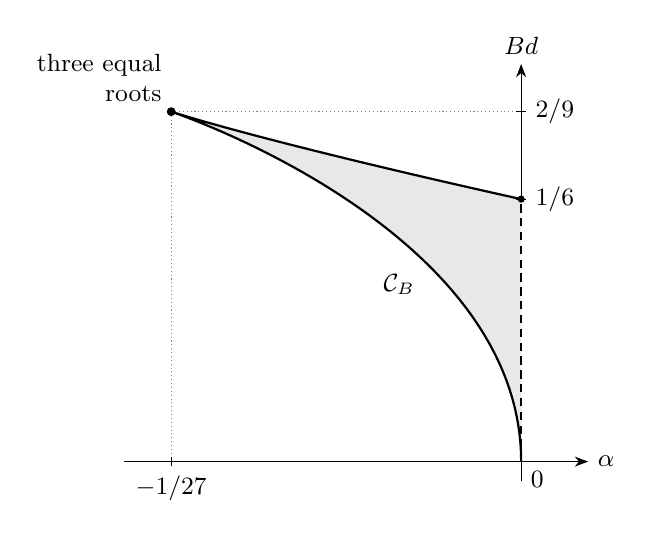
\begin{tikzpicture}[x=1cm,y=1cm,>=Stealth,font=\small]
\fill[black!9] plot[domain=0:0.5,samples=181,variable=\t]
 ({-120*\t*\t*(1-2*\t)},{(40/3)*(2*\t-3*\t*\t)}) -- (0,0) -- cycle;
\draw[->] (-5.05,0)--(0.85,0) node[right]{$\alpha$};
\draw (0,-0.25)--(0,0);
\draw[->] (0,{10/3})--(0,5.05) node[above]{$B d$};
\draw[thick] plot[domain=0:0.5,samples=181,variable=\t]
 ({-120*\t*\t*(1-2*\t)},{(40/3)*(2*\t-3*\t*\t)});
\draw[thick,densely dashed] (0,0)--(0,{10/3});
\draw[black!50,densely dotted] ({-40/9},{40/9})--(0,{40/9});
\draw[black!50,densely dotted] ({-40/9},0)--({-40/9},{40/9});
\draw ({-40/9},0.06)--({-40/9},-0.06) node[below]{$-1/27$};
\draw (-0.06,{40/9})--(0.06,{40/9}) node[right]{$2/9$};
\draw (-0.06,{10/3})--(0.06,{10/3}) node[right]{$1/6$};
\fill ({-40/9},{40/9}) circle(1.6pt);
\fill (0,{10/3}) circle(1.3pt);
\node[above left,align=right] at ({-40/9},{40/9}) {three equal\\roots};
\node at (-1.55,2.25) {$\mathcal C_B$};
\node[below right] at (0,0) {$0$};
\end{tikzpicture}

\caption{The secondary corner of the principal-scale saturation domain, in coordinates \((\alpha,Bd)\).
The shaded interior corresponds to three distinct positive roots of
\(z^3-z^2+(3Bd/2)z+\alpha\). The solid boundary has a repeated root;
the dashed segment has a zero root. The dot at
\((-1/27,2/9)\) has three equal roots. The solid curve is
\((\alpha,Bd)=(-t^2(1-2t),2(2t-3t^2)/3)\), \(0\le t\le1/2\).
}
\label{fig:corner-limit-set}
\end{figure}

\begin{proof}[Proof of Proposition~\ref{corner:complete-cluster-set}]
Boundedness of $\alpha,d$ follows from
Proposition~\ref{corner:secondary-bounds}, so consider any cluster point.
For $d_0>0$, Lemma~\ref{corner:limiting-critical-states} gives
a cubic with positive critical states $z_-\leq z_+$,
nonnegative maximum, nonpositive minimum, and
$F_{\alpha_0,d_0}(0)=\alpha_0\leq0$.  Hence it has three
nonnegative real roots, counted with multiplicity.  This conclusion
includes equality of critical values or $\alpha_0=0$ by continuity,
or directly by the intermediate value theorem on the intervals
$[0,z_-]$, $[z_-,z_+]$, and $[z_+,\infty)$.
At $T_{3,0}=1/3$ the two critical states coincide; their two
value inequalities force a triple root there.
For $d_0=0$ the limiting polynomial is $z^2(z-1)$.
In every case Vieta's identities give membership in $\mathcal C_B$.

The discriminant of $z^3-z^2+T_3 z+\alpha$ is the expression
in \eqref{corner:discriminant}.  Conversely, that discriminant and
$\alpha\leq0$, $T_3\geq0$ give three real roots with sum one,
nonnegative product, and nonnegative pair sum.  If a root were
negative, the product condition would allow us to write the two
nonpositive roots as $-u,-v$, with $u>0$, $v\geq0$, and the third
as $1+u+v$.  Their pair sum would be
$-u^2-uv-v^2-u-v<0$, a contradiction.  This proves
\eqref{corner:discriminant}.  Strict positivity and distinctness
characterize the interior; a zero root or a repeated root is on its
boundary.

For nonnegative $r_i$ with sum one,
$r_1r_2r_3\leq1/27$ and
$r_1r_2+r_1r_3+r_2r_3\leq1/3$.
These inequalities prove \eqref{corner:sharp-cluster-bounds}.
Equality in the second requires $r_1=r_2=r_3=1/3$ and gives the
stated top endpoint.  If $a\geq0$ eventually, every cluster point
has $\alpha_0=0$.  Its polynomial is
$z(z^2-z+T_{3,0})$, whose two remaining roots are real and
nonnegative only if $T_{3,0}\leq1/4$.  This proves
\eqref{corner:nonnegative-offset-bound}.

For the interior converse, fix a compact
$\mathcal K\Subset\operatorname{int}\mathcal C_B$. The ordered positive
roots $r_j$ have uniform positive lower bounds, pairwise
separation, and nonzero derivative margins.  Lemma
\ref{corner:joint-quotient} transfers them to three simple roots on
disjoint positive $z$-intervals for every independently small positive
$\mu,\sigma$, uniformly on $\mathcal K$. The other three roots follow from the
charts of Lemma~\ref{corner:realization-charts}.  The first chart has its
negative root at $x=\alpha$, the second at $X=1$, and the third at
$X=1/C^2$, all with strict uniform derivative margins.
The negative secondary root and the three positive secondary roots
have size $\mu^2\sigma^2$, whereas the outer negative root has size
$\mu^2\sigma$ and the outer positive root size $\mu^2$. The six isolating
intervals are therefore disjoint for small $\sigma$.
All their states belong to $I$ for small scales.

The standard unfolding realizes \eqref{corner:weights} on one product
$(0,\mu_0)\times(0,\sigma_0)$ for $\mathcal K$,
and~\cite[Proposition~\ref*{main-prop:common-count}]{main2026} makes the six
simple roots exhaustive; the same charts give \eqref{corner:interior-roots}.

For any boundary point, convexly perturb its ordered root triple toward
$(1/6,1/3,1/2)$ to obtain interior parameters $(\alpha_j,d_j)$ tending
to it. For the $j$th interior parameter choose
positive $\mu_j,\sigma_j<1/j$ below the two existence thresholds
just proved.  The corresponding return map has six simple roots,
and its normalized parameters are exactly $(\alpha_j,d_j)$.
This proves the diagonal assertion and, together with necessity,
identifies the full cluster set as $\mathcal C_B$.
It also proves sharpness of the unrestricted cluster bounds.

\end{proof}

\subsection{Hausdorff convergence}

To obtain convergence of the full domains, we first place the normalized
parameters of all six-cycle returns in one common rectangle.
For the standard unfolding and the $\mathcal V,I$ of
Definition~\ref{def:actual-secondary-domain},
Proposition~\ref{corner:secondary-bounds} bounds the full local domain by
$-K\le\alpha\le K\mu^2$ and $0<d\le K$. Choose
$\mathcal B=[-M,M]^2$, $M>K$, containing $\mathcal C_B$ in its interior.
The weighted parameters~\eqref{corner:weights} tend uniformly
to zero on this rectangle for independently small positive scales. Thus
$\Lambda\circ w_{\mu,\sigma}$ is defined throughout $\mathcal B$ after
one common reduction, and
$\mathscr S_{\mu,\sigma}\subset\operatorname{int}\mathcal B$.
The rectangle therefore contains the normalized parameters of every six-cycle
return in $\mathcal V$, including those with positive offset.

\begin{proof}[Completion of Proposition~\ref{thm:saturation-geometry}]
We apply the compactness and finite-net argument that completes the proof
of~\cite[Theorem~\ref*{main-thm:main-saturation-summary}]{main2026} in
\cite[Section~\ref*{main-subsec:four-root-limit}]{main2026}. The common rectangle above makes
every closure compact. An interior singleton of $\mathcal C_B$ is realized
by part~2 of
Proposition~\ref{corner:complete-cluster-set} for every sufficiently small
independent scale pair, so these closures are nonempty.

For the upper inclusion, the weighted parameters tend uniformly to the fixed
reference on $\mathcal B$, so part~1 applies along arbitrary sequences
$\mu_n,\sigma_n\to0^+$. For the lower inclusion, the root perturbation
above gives interior density. Every finite interior net is compact, so
part~2 realizes it in the standard unfolding on one product of positive
scale intervals, with no relation between the scales. These are the
two-scale inputs to the cited argument, which gives both Hausdorff inclusions.
\end{proof}

\section{Optimal positive closing offset and its realization}\label{sup:positive}

Here positive offset means $a=R(0)>0$.
The constructions below use the finer offset scale $a=\eta h^3$, with
$\alpha=\eta\mu^2>0$ and $\alpha\to0$; the limiting cubic region
$\mathcal C_B$ has $\alpha\le0$.
Two positive roots precede the second threshold and two persist on the
secondary scale.
The realization below adds the outer negative and positive roots to these
two clusters; the bound of six then excludes further roots in $I$.

\begin{proposition}[Positive-offset six-cycle returns]
\label{corner:positive-offset-realization}
\label{thm:positive-offset-six}
Assume~\cite[(\ref*{main-eq:rank})]{main2026} and use the standard
unfolding on $I$.
Put
\[
 \eta_*=\frac{4}{27B^2},\qquad d_*=\frac{1}{6B}.
\]
For every compact
$\mathcal K\Subset(0,\eta_*)\times(0,d_*)$, there are
$\mu_0,\sigma_0>0$ such that the parameters
\begin{equation}\label{corner:positive-offset-weights}
 m=\mu,\qquad h=\mu^2\sigma,\qquad b=-h,\qquad
 \delta=\mu^3\sigma^2d,\qquad a=\eta h^3
\end{equation}
give exactly one negative and five positive simple fixed points in $I$
for every
\[
 0<\mu<\mu_0,\qquad0<\sigma<\sigma_0,\qquad
 (\eta,d)\in\mathcal K.
\]

Let $u_-(\eta)<u_+(\eta)$ be the two positive roots of
$\eta-z^2+Bz^3$, and put
\[
 r_\pm(d)=\frac{1\pm\sqrt{1-6Bd}}2.
\]
The six states satisfy, uniformly on $\mathcal K$,
\begin{align}
 q_N&=-\frac hC(1+o(1)),\notag\\
 q_{F,\pm}&=h^2\bigl(u_\pm(\eta)^2+o(1)\bigr),\notag\\
 q_{S,\pm}&=\mu^2\sigma^2\bigl(r_\pm(d)^2+o(1)\bigr),\notag\\
 q_O&=\frac{\mu^2}{C^2}(1+o(1)).
                                  \label{corner:positive-offset-roots}
\end{align}
Here $o(1)\to0$ as $\mu+\sigma\to0$, with the positive scales
independent. The constants $\eta_*$ in
\eqref{corner:sharp-positive-offset-limsup} and $d_*$ in
\eqref{corner:nonnegative-offset-bound} are sharp: both are approached
simultaneously by a sequence of these positive-offset returns.
\end{proposition}

\begin{proof}
Uniform convergence of \eqref{corner:positive-offset-weights} to zero
on $\mathcal K$ lets the standard unfolding realize them on one
product of scale intervals.

Below the second threshold $a_\delta=\Gamma_1^{-1}(\delta)$, the passage
and closing expansions give
\begin{equation}\label{corner:positive-first-only-identity}
 D(r^2)=a-hr^2+kA_1(\lambda)r^3+r^4T(r,\lambda),
 \qquad k=1-h,
\end{equation}
where $T$ is jointly smooth on a common signed-root domain.
For $r=hz$ on a compact positive $z$ interval,
\[
 \frac{\Gamma_1(h^2z^2)}{\delta}
   =\frac{\mu z^2}{d}\{1+O(h)\}.
\]
Thus only the first passage is active at these states for all sufficiently
small $\mu$,
uniformly on $\mathcal K$ and independently of $\sigma$. Their
normalized displacement satisfies
\begin{equation}\label{corner:positive-first-only-limit}
 \frac{D(h^2z^2)}{h^3}
 =\eta-z^2+kA_1(\lambda)z^3+hz^4T(hz,\lambda)
 =\eta-z^2+Bz^3+O_{C^1}(\mu).
\end{equation}
Indeed the standard unfolding gives $A_1(\lambda)-B=O(\mu)$ on a bounded
rectangle of scales, and the smooth root formula controls the displayed
remainder and its $z$ derivative.

The limiting polynomial is positive at zero and at infinity.
Its positive critical point at $2/(3B)$ is a minimum, with value
$\eta-\eta_*<0$.
It therefore has two positive simple roots $u_\pm(\eta)$.

The secondary weights \eqref{corner:weights} now have
$\alpha=\eta\mu^2>0$. Substitution in the joint quotient
\eqref{corner:joint-limit} gives, on compact positive $z$ intervals,
\begin{equation}\label{corner:positive-secondary-limit}
 \frac{D(\mu^2\sigma^2z^2)}{\mu^4\sigma^3}
 =z\bigl(z^2-z+\tfrac32Bd\bigr)+O_{C^1}(\mu+\sigma).
\end{equation}
For $0<d<d_*$, its two nonzero limiting roots $r_\pm(d)>0$ have
derivatives $r_\pm(2r_\pm-1)\ne0$. Both passages are active on their
isolating intervals because
\[
 \frac{a_\delta}{\mu^2\sigma^2z^2}
   =\frac{\mu d}{z^2}\{1+o(1)\}\longrightarrow0
\]
uniformly on their isolating intervals.

Finally apply the outer charts
\eqref{corner:negative-large-chart} and
\eqref{corner:positive-large-chart} with $\alpha=\eta\mu^2$.
Their $C^1$ limits $X-X^2$ and $X^{3/2}-CX^2$ have simple roots at
$1$ and $1/C^2$.

All four joint $C^1$ chart limits have compact isolating intervals with uniform
derivative margins on $\mathcal K$. Simple-root continuation gives the
six roots in \eqref{corner:positive-offset-roots} for common
thresholds $\mu_0,\sigma_0$, without a relation between the positive
scales. The windows where only the first passage is active have size
$h^2=\mu^4\sigma^2$, the secondary windows size $\mu^2\sigma^2$,
and the positive outer window size $\mu^2$. Their successive ratios
are $O(\mu^2)$ and $O(\sigma^2)$; the negative window is separated
by sign. The second threshold lies strictly between the first-passage and
secondary windows. All six windows lie in $I$ for small scales,
and~\cite[Proposition~\ref*{main-prop:common-count}]{main2026} excludes
additional fixed points there. The charts also give
\eqref{corner:positive-offset-roots}.

For sharpness choose interior pairs $(\eta_j,d_j)$ tending to
$(\eta_*,d_*)$. Apply the result to each singleton pair and choose
positive $\mu_j,\sigma_j<1/j$ below its two existence thresholds.
The resulting returns have exactly
\[
 \frac{a_j}{h_j^3}=\eta_j\longrightarrow\eta_*,
 \qquad
 \frac{m_j\delta_j}{h_j^2}=d_j\longrightarrow d_*.
\]
\end{proof}

\begin{corollary}[Six-cycle regions with positive offset]
\label{corner:open-six-cycle-region}
\label{cor:six-open}
By~\cite[Corollary~\ref*{main-cor:six-open}]{main2026}, in every admissible
family the parameters giving six simple fixed points in $I$ form an open
set. Under~\cite[(\ref*{main-eq:rank})]{main2026}, this set contains open
subsets with $a>0$, one negative fixed point and five positive fixed points,
accumulating at the reference.
\end{corollary}

\begin{proof}
The openness assertion
is~\cite[Corollary~\ref*{main-cor:six-open}]{main2026}.
For the returns of Proposition~\ref{corner:positive-offset-realization},
shrink the neighbourhood to preserve $a>0$ and the signs of the six
simple roots. An interior parameter pair with both scales tending to zero
gives accumulation at the reference.
\end{proof}

\section{The secondary cusp on the whole interval}\label{sup:cusp}

We first separate the secondary triple-root cluster from the three simple
roots on the rest of the interval $I$. This localization supplies the
complete cycle count when the cluster is unfolded.

\subsection{Location of all roots near the secondary triple root}

\begin{lemma}[All roots near the secondary triple root]
\label{corner:all-roots}
Use the standard unfolding.
Fix a sufficiently small interval $J=(z_-,z_+)\ni1/3$.
There are a neighbourhood $\mathcal U$ of
$(-1/27,2/(9B))$, with compact closure in $\{\alpha<0,d>0\}$,
and $\mu_0,\sigma_0>0$ such that the following statements hold for every
\[
 (\alpha,d)\in\overline{\mathcal U},\qquad
 0<\mu<\mu_0,\qquad 0<\sigma<\sigma_0.
\]
Then $P''$ has exactly two simple zeros $\zeta_1<\zeta_2$ in the outer region,
with
\begin{equation}\label{corner:independent-curvature-roots}
 \sqrt{\zeta_1}=\mu\sigma\{\sqrt{Bd/2}+O(\mu+\sigma)\},\qquad
 \sqrt{\zeta_2}=\mu\{3/(8C)+O(\mu+\sigma^2)\}.
\end{equation}
The interval $\mathcal J=\{\mu^2\sigma^2z^2:z\in J\}$ contains
$\zeta_1$ and lies strictly between the second threshold and $\zeta_2$.
Outside $\mathcal J$ the displacement has exactly three roots,
all simple, with uniform asymptotics
\begin{equation}\label{corner:cusp-companions}
\begin{aligned}
 q_{N,1}&=-\frac{\mu^2\sigma}{C}(1+o(1)),&
 q_{N,2}&=\mu^2\sigma^2(\alpha+o(1)),\\
 q_{P,\mathrm{out}}&=\frac{\mu^2}{C^2}(1+o(1)).
\end{aligned}
\end{equation}
Inside $\mathcal J$ there are between one and three distinct roots.
All limits are uniform as $\mu+\sigma\to0$, without a condition on
the ratio of the two scales.
\end{lemma}

\begin{proof}
Use the separation graph~\eqref{corner:curvature-division} with
$p=(a,b,\xi_0)$. Substitution of $r=\mu\sigma z_g$ gives
\[
 d=z_g^2\{H_\Delta(\mu\sigma z_g,\mu,p)
                   +\sigma z_g B_\Delta(\mu\sigma z_g,p)\}.
\]
At zero scales the positive solution is $z_g=\sqrt{Bd/2}$, and the
state derivative of the right side is $4z_g/B>0$.
Substitution of $r=\mu w_g$ instead gives
\[
 \sigma^2d=w_g^2\{H_\Delta(\mu w_g,\mu,p)+w_gB_\Delta(\mu w_g,p)\}.
\]
Its nonzero positive solution at zero scales is $w_g=3/(8C)$; the
state derivative there is $-3/(4BC)$. The parameter implicit function
theorem proves~\eqref{corner:independent-curvature-roots} uniformly on
a compact neighbourhood of the parameters. In the second equation the restriction
at $\mu=0$ depends on $\sigma$ only through $\sigma^2d$, giving the
stated remainder. Both roots are in the outer region, since
$\delta/\zeta_1=O(\mu)$ and $\delta/\zeta_2=O(\mu\sigma^2)$.
The graph with its unique positive critical point and the threshold-layer
estimate of~\cite[Lemma~\ref*{main-lem:event-layer}]{main2026} exhaust the
interval and exclude any other zero of $P''$. These two simple zeros and the threshold-layer signs give
\[
\begin{array}{c|ccccc}
q&(-q_0,0)&(0,a_\delta)&(a_\delta,\zeta_1)&(\zeta_1,\zeta_2)&(\zeta_2,q_0)\\ \hline
\sgn D_{qq}&-&+&-&+&-
\end{array}
\]
where $a_\delta=\Gamma_1^{-1}(\delta)$.

The threshold identities $Q(a_\delta)=\delta$ and
$a_\delta=\delta-A_1\delta^{3/2}+O(\delta^2)$ yield
\[
 D(a_\delta)-a=b\delta+A_1\delta^{3/2}+O(\delta^2),\qquad
 \frac{D(a_\delta)}{\mu^4\sigma^3}=\alpha+O(\sqrt\mu).
\]
Indeed the three normalized errors are respectively
$O(\mu)$, $O(\sqrt\mu)$ and $O(\mu^2\sigma)$.
Thus $D(0)<0$ and $D(a_\delta)<0$ uniformly. Strict convexity on $(0,a_\delta)$
excludes all roots between and at the thresholds.

Choose $J=(1/3-\varepsilon,1/3+\varepsilon)$ with $\varepsilon>0$
fixed and small. At the central parameters the zero-scale quotient is
$(z-1/3)^3$. Its endpoint values are $\pm\varepsilon^3$ and its
endpoint derivatives are $3\varepsilon^2$. First shrinking
$\mathcal U$, then the common scale rectangle, gives
\begin{equation}\label{corner:cusp-window-signs}
 \mathcal F(z_-)<0<\mathcal F(z_+),\qquad
 \mathcal F_z(z_\pm)>0.
\end{equation}
Write $q_\pm=\mu^2\sigma^2z_\pm^2$. The curvature locations and
$a_\delta\sim\delta$ give $a_\delta<q_-<\zeta_1<q_+<\zeta_2$.
In particular,
\[
 D(q_-)<0<D(q_+),\qquad
 D_q(q_\pm)=\frac{\mu^2\sigma}{2z_\pm}
                       \mathcal F_z(z_\pm)>0.
\]
On $(a_\delta,q_-)$ the derivative is decreasing and hence positive, so
$D<D(q_-)<0$. On $(q_+,\zeta_2)$ it is increasing and positive, so
$D>D(q_+)>0$, including $D(\zeta_2)>0$.

Lemma~\ref{corner:realization-charts} gives one simple root near each
of $x=\alpha$, $X=1$, and $X=1/C^2$ in its three charts. Their
nonzero limiting derivatives have common margins on
$\overline{\mathcal U}$, and their isolators are disjoint for small
$\sigma$. This proves~\eqref{corner:cusp-companions}.
The negative half-interval is strictly concave and therefore has at most
two zeros, so the two negative roots exhaust it. The outer positive
root lies beyond $\zeta_2$, since $1/C>3/(8C)$, and has
$D_q=\mu^2\{-1/(2C)+o(1)\}<0$. Strict concavity on $(\zeta_2,q_0)$,
starting at the positive value $D(\zeta_2)$, keeps $D$ positive before
this root and negative after it. This excludes every other root up
to the fixed right endpoint. The negative-side concavity likewise
covers its entire fixed tail.

Only $\mathcal J$ remains. Its endpoint values have opposite signs,
and its only zero of $P''$ is $\zeta_1$, with negative curvature before
and positive curvature after it. Thus $D_q$ has at most two zeros there,
and Rolle's theorem gives at most three roots. All comparisons above
use separate small bounds on $\mu$ and $\sigma$ on the same interval.
\end{proof}

\subsection{The cusp and its fold curves}

Lemma~\ref{corner:all-roots} places the secondary cluster where both passages
are active, with three simple roots on the rest of $I$. We apply the
preparation theorem to the joint quotient of
Lemma~\ref{corner:joint-quotient}.

\begin{theorem}[Cusp and cycle counts]\label{thm:actual-cusp}
For the standard unfolding, there are a neighbourhood
$\mathcal U\ni(-1/27,2/(9B))$ and $\mu_0,\sigma_0>0$
such that the following hold on $\mathcal U$ for every independent pair
$0<\mu<\mu_0$, $0<\sigma<\sigma_0$. There is a unique nearby
jointly smooth branch $(\alpha_c,d_c,z_c)(\mu,\sigma)$ of triple zeros
of $\mathcal F_{\mu,\sigma}$ through
$(-1/27,2/(9B),1/3)$ at zero scales.
The separation $\delta_{\rm cusp}=\mu^3\sigma^2d_c$ and
state $q_{\rm cusp}=\mu^2\sigma^2z_c^2$ give a limit cycle of multiplicity
three.

In the normalized variables $(\mu,\sigma,z,\alpha,d)$ there are jointly
smooth changes of state and parameters, with a nonzero smooth factor, which
reduce the local zero equation to
\begin{equation}\label{corner:cusp-preparation}
 y^3+uy+v=0.
\end{equation}
For each positive $\mu,\sigma$, $(u,v)$ are local coordinates on the slice
$m=\mu$, $b=-\mu^2\sigma$ of the standard unfolding. Throughout $\mathcal U$,
the prepared coordinates give the following counts in $I$:
four simple cycles when $4u^3+27v^2>0$ and six simple cycles when
$4u^3+27v^2<0$. Both regions are nonempty and open. On the fold arcs
$4u^3+27v^2=0$, $(u,v)\ne(0,0)$, there are five distinct cycles,
one double; at $(u,v)=(0,0)$ there are four distinct cycles, one triple.

In the rescaled parameters $(\alpha,d)$ the double-root curve is obtained
by solving
\begin{equation}\label{corner:actual-fold-curve}
 \mathcal F(t;\alpha_f,d_f)=0,\qquad
 \mathcal F_z(t;\alpha_f,d_f)=0
\end{equation}
for $(\alpha_f,d_f)$, with $t$ near $1/3$.
The curve has an ordinary cusp at $t=z_c$ and consists
of two ordinary fold arcs away from that point.
\end{theorem}

\begin{proof}
At $(\mu,\sigma,\alpha,d,z)=(0,0,-1/27,2/(9B),1/3)$,
the quotient is $(z-1/3)^3$, and
\[
 D_{(\alpha,d,z)}(\mathcal F,\mathcal F_z,\mathcal F_{zz})
 =\begin{pmatrix}1&B/2&0\\0&3B/2&0\\0&0&6\end{pmatrix},
 \qquad \det=9B.
\]
The parameter implicit function theorem gives the jointly smooth branch,
which differs from its limiting value by $O(\mu+\sigma)$ and has
$\mathcal F_{zzz}=6+O(\mu+\sigma)>0$.
Moreover
\[
 \frac{q_{\rm cusp}}{\delta_{\rm cusp}}
 =\frac{z_c^2}{\mu d_c}
 =\frac B{2\mu}\{1+O(\mu+\sigma)\}\longrightarrow\infty.
\]
Since the second threshold is asymptotic to $\delta_{\rm cusp}$, both
passages are active at the triple root and $D$ is smooth in $q$ there; the
state change $q=\mu^2\sigma^2z^2$ preserves multiplicity.

The Malgrange preparation theorem~\cite[Chapter~IV, Section~2, Theorem~2.1 and Note~(1), p.~95]{golubitsky1973}, with
both scales as parameters, followed by removal of the quadratic term gives
\eqref{corner:cusp-preparation}. At zero scales, with
$\widehat\alpha=\alpha+1/27$ and $\widehat d=d-2/(9B)$,
\[
\begin{aligned}
 u&=\tfrac32B\widehat d+O((|\widehat\alpha|+|\widehat d|)^2),\\
 v&=\widehat\alpha+\tfrac B2\widehat d
                         +O((|\widehat\alpha|+|\widehat d|)^2).
\end{aligned}
\]
At zero scales the parameter Jacobian is $-3B/2\ne0$, so it remains
nonzero on a common reduction.
Choose $J$ of Lemma~\ref{corner:all-roots} inside the preparation chart,
then reduce the parameters and the rectangle of scales so that every prepared
cubic root pulls back into $J$. The cubic discriminant gives one or
three simple roots on its two open sides, two distinct roots on a
nonzero fold, and a triple root at the origin. Both open sides occur
because the parameter change is a local diffeomorphism. Adding the three
simple roots of Lemma~\ref{corner:all-roots} gives all stated counts
on $I$.

For the fold curve, the equations
$(\mathcal F,\mathcal F_z)=0$ at $z=t$ have parameter Jacobian
\[
 D_{(\alpha,d)}(\mathcal F,\mathcal F_z)
 =\begin{pmatrix}1&3Bt/2\\0&3B/2\end{pmatrix}
 \quad\hbox{at zero scales}.
\]
The uniform implicit function theorem gives jointly smooth functions
$(\alpha_f,d_f)$ on a compact $t$ interval, with zero-scale curve
$\alpha_0(t)=-t^2+2t^3$, $d_0(t)=2t(2-3t)/(3B)$.
Differentiating the fold equations gives $\gamma_f'(z_c)=0$ for
$\gamma_f=(\alpha_f,d_f)$, since their parameter Jacobian is invertible
and $\mathcal F_z=\mathcal F_{zz}=0$ there. Smooth dependence on the
scales and the zero-scale curve give
\begin{equation}\label{corner:ordinary-cusp-determinant}
 \det\bigl(\gamma_f''(z_c),\gamma_f'''(z_c)\bigr)
       =\frac{48}{B}+O(\mu+\sigma)\ne0.
\end{equation}
Thus $\gamma_f$ has an ordinary cusp. Along it,
$\frac{d}{dt}\mathcal F_{zz}=\mathcal F_{zzz}>0$ at the cusp;
after a common reduction all other points are ordinary double roots.
\end{proof}

Figure~\ref{fig:cusp-local-diagram} shows the cycle counts on $I$ in the
prepared coordinates.
% Discriminant of the prepared cubic y^3+uy+v.
% Curve parameter: (u,v)=(-3t^2,2t^3).
% The homogeneous rescaling (u,v)=(eta^2 U,eta^3 V)
% puts this drawing inside an arbitrarily small prepared-control chart.
% Source and independent polynomial checks: scripts/check-secondary.py.
\begin{figure}[!htbp]
\centering
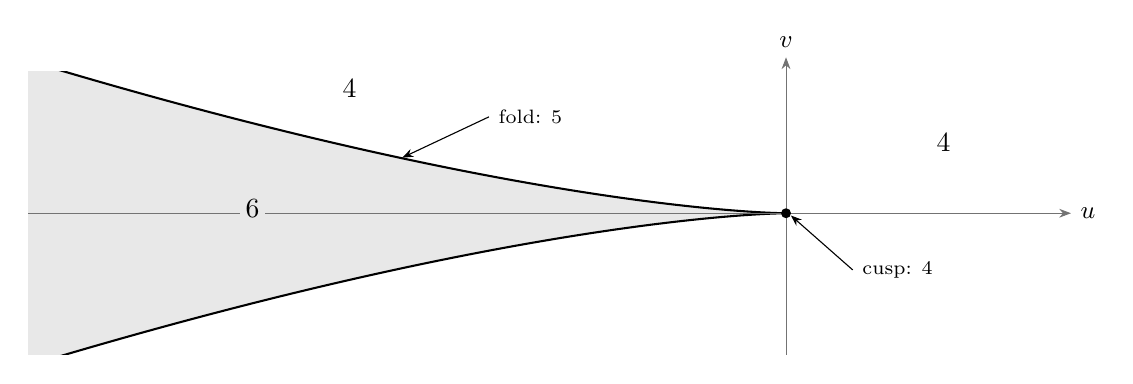
\begin{tikzpicture}[x=7.7cm,y=3.6cm,font=\small,
  boundary/.style={black,line width=.75pt},
  guide/.style={black!55,line width=.35pt},
  leader/.style={black,line width=.4pt,-{Stealth[length=1.4mm]}},
  region/.style={fill=white,inner sep=2pt,font=\normalsize}]
  \begin{scope}
    \clip (-1.25,-.50) rectangle (.42,.50);
    \fill[black!9]
      plot[domain=-.67:.67,variable=\t,samples=181]
        ({-3*(\t)^2},{2*(\t)^3}) -- cycle;
    \draw[boundary]
      plot[domain=-.67:.67,variable=\t,samples=181]
        ({-3*(\t)^2},{2*(\t)^3});
  \end{scope}
  \draw[guide,-{Stealth[length=1.5mm]}]
    (-1.25,0)--(.47,0) node[right,black] {$u$};
  \draw[guide,-{Stealth[length=1.5mm]}]
    (0,-.50)--(0,.55) node[above,black] {$v$};
  \node[region,fill=black!9] at (-.88,.015) {$6$};
  \node[region] at (.26,.25) {$4$};
  \node[region] at (-.72,.44) {$4$};
  \node[anchor=west,font=\scriptsize] (fold) at (-.49,.34) {fold: $5$};
  \draw[leader] (fold.west)--(-.633,.196);
  \fill (0,0) circle[radius=1.8pt];
  \node[anchor=west,font=\scriptsize] (cusp) at (.11,-.20) {cusp: $4$};
  \draw[leader] (cusp.west)--(.008,-.008);
\end{tikzpicture}
\caption{The cusp in the prepared coordinates of
$y^3+uy+v=0$. The boundary is $4u^3+27v^2=0$:
the shaded region has six simple cycles and the other region has four,
including the three simple cycles outside the local cluster.
An ordinary fold has five different cycles, one double; the cusp has four,
one triple. A sufficiently small weighted rescaling of $(u,v)$ places the
diagram inside the common local parameter neighbourhood.
The pullback of the discriminant to $(\alpha,d)$ is the local bifurcation
curve, including its cusp.}
\label{fig:cusp-local-diagram}
\end{figure}


\section*{Acknowledgments and AI tool disclosure}

OpenAI’s ChatGPT and Codex were used during the development and preparation of this work. These tools assisted with exploring proof strategies, developing and checking mathematical arguments, preparing verification scripts, and revising the exposition and LaTeX source. They were also used to help identify relevant literature and potential gaps in intermediate drafts. The author is responsible for the mathematical claims, references, and final presentation of the paper.

\section*{Statements and Declarations}

\paragraph{Funding.}
The author received no funding for this work.

\paragraph{Competing interests.}
The author has no competing interests to declare.

\paragraph{Author contributions.}
Haibo Lu was responsible for the research design, mathematical analysis,
computational verification, and writing and revision of the manuscript.

\paragraph{Data and code availability.}
This document is Online Resource~1. Its editable source and finite secondary
polynomial checker accompany this paper. Online Resource~2
contains the separate symbolic verification package; Online Resource~3
contains computer-assisted proofs that, at each of two fixed parameter tuples, the
harvesting model has at least six distinct simple periodic orbits.
The analytic results are proved in the text; the computational files
provide independent checks and fixed-parameter examples.

\begin{thebibliography}{9}
\setlength{\itemsep}{1pt}

\bibitem{main2026}
H.~Lu,
Cyclicity Six and Saturation Geometry at Cancelling Double Grazing,
accompanying manuscript.

\bibitem{dibbc2001}
M.~di Bernardo, C.~J.~Budd and A.~R.~Champneys,
Normal form maps for grazing bifurcations in \(n\)-dimensional
piecewise-smooth dynamical systems,
\emph{Physica D} \textbf{160} (2001), 222--254.
\url{https://doi.org/10.1016/S0167-2789(01)00349-9}.

\bibitem{nordmark2002}
A.~B.~Nordmark,
Discontinuity mappings for vector fields with higher order continuity,
\emph{Dynamical Systems} \textbf{17} (2002), 359--376.
\url{https://doi.org/10.1080/1468936021000041645}.

\bibitem{golubitsky1973}
M.~Golubitsky and V.~Guillemin,
\emph{Stable Mappings and Their Singularities},
Graduate Texts in Mathematics \textbf{14}, Springer, New York, 1973.
\url{https://doi.org/10.1007/978-1-4615-7904-5}.

\bibitem{simpsonmeiss2008}
D.~J.~W.~Simpson and J.~D.~Meiss,
Unfolding a codimension-two, discontinuous, Andronov--Hopf bifurcation,
\emph{Chaos} \textbf{18} (2008), article 033125.
\url{https://doi.org/10.1063/1.2976165}.
\href{https://arxiv.org/abs/0804.3101}{arXiv:0804.3101}.

\end{thebibliography}

\end{document}
